\chapter{ Sprint 2 : Reward System}

\setcounter{secnumdepth}{0}
\phantomsection
\section{Introduction}
In this chapter, we will delve into the planning, design, and implementation of our reward system. This system aims to enhance user engagement by awarding tokens and XP for specific actions and achievements. We will explore requirements gathering, static and dynamic modeling, microservices communication, and the use of RabbitMQ as our message broker. Through this comprehensive approach, we ensure a robust and scalable reward mechanism that aligns with our project goals.\setcounter{secnumdepth}{3} 
\section{Requirements Gathering}
By conducting a comprehensive analysis of the requirements, we aim to bridge the gap between the stakeholders’ vision and the actual implementation of the reward system. This analysis helps us define clear and concise specifications that serve as the foundation for the design, development, and testing phases of the project.

\subsection{Identifying End-Users}
Identifying end-users is a crucial step in requirements analysis as it helps determine the needs, expectations, and constraints of the target audience. In our reward system, we have identified two types of actors:

\begin{itemize}
    \item \textbf{Administrator:} Responsible for overseeing user accounts, configuring, and maintaining the reward system to ensure smooth operation.
    \item \textbf{Subcontractor:} Engages with the reward system by earning tokens and XP through various activities and managing their achievements.
\end{itemize}

\subsection{Functional Requirements}
Functional requirements define the specific actions, tasks, and behaviors that the reward system must be able to perform to meet the needs of its end-users. These requirements form the foundation of the system’s functionality.The functional requirements captured for each actor are outlined below.

\subsubsection*{Authentication and Profile Settings}
\begin{itemize}
    \item \textbf{Sign in:} A registered user should be able to access the system by providing valid credentials.
    \item \textbf{Edit profile settings:} A logged-in user should be able to edit their profile settings.
\end{itemize}

\subsubsection*{Administrator Requirements}
\begin{itemize}
    \item \textbf{Manage Achievements:} An administrator should be able to update and list achievements.
    \item \textbf{Manage Tokens and XP:} An administrator should be able to list tokens and XP, edit tokens and XP, increment and decrement tokens, and ban/unban users from gaining tokens.
    \item \textbf{Manage Transactions:} An administrator should be able to view all transactions for a specific user.
    \item \textbf{Manage Ranks:} An administrator should be able to view ranks, levels, and next rank for each user.
\end{itemize}

\subsubsection*{Subcontractor Requirements}
\begin{itemize}
    \item \textbf{View Achievements:} A subcontractor should be able to view all possible achievements in the application.
    \item \textbf{View Tokens and XP:} A subcontractor should be able to view their tokens and XP.
    \item \textbf{Close Packet:} A subcontractor should be able to gain tokens and XP by closing a packet.
    \item \textbf{User Features:} An administrator should be able to view the FAQ and Shop pages.
\end{itemize}

\section{Scrum Implementation Overview}
This section provides an overview of the Scrum implementation in our project. It includes a global use case diagram, showcasing the system’s high-level functionalities, followed by the presentation of the product backlog and the planning of the sprints.

\subsection{Global Use Case Diagram}
Using UML use case diagrams provides a clear visual representation of actor-system interactions and concisely specifies expected functionalities and behaviors. The figure \ref{fig:global_use_case} illustrates the global use case diagram we modeled for our reward system.

\begin{figure}[H]
    \centering
    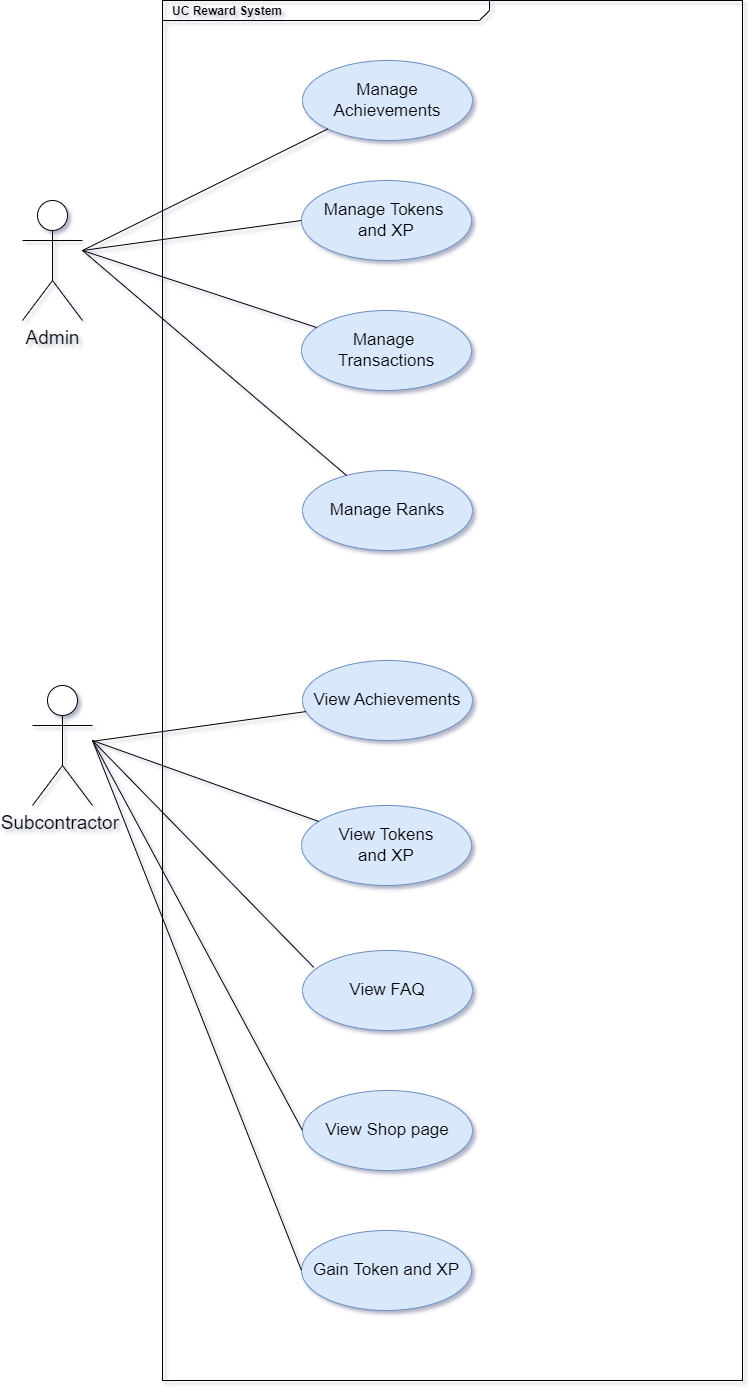
\includegraphics[width=0.5\textwidth]{src/assets/diagrams/GlobalUseCaseUC.png}
    \caption{Global Use Case Diagram for Reward System}
    \label{fig:global_use_case}
\end{figure}

\section{Sprint backlog}
During the Sprint Planning meeting, the effort for each task in the first and second sprint backlogs was assessed based on the total working hours required. The prioritization of these backlog items is depicted through their sequence in the table, with items placed at the top representing higher urgency.  accompanying image showcases the board t
 \\
\begin{longtable}{ | m{0.08\textwidth}  | m{0.18\textwidth} | m{0.39\textwidth} | c | }
    \caption{Backlog of Sprint 2}                                                                                                          \\
    \hline
    \textbf{Sprint}         & \textbf{Epic}                                        & \textbf{User story}          & \textbf{Estimation (hours)} \\
    \hline
    \endfirsthead
    \hline
    \textbf{Sprint}         & \textbf{Epic}                                        & \textbf{User story}          & \textbf{Estimation (hours)} \\
    \hline
    \endhead
    \hline
    \endfoot
    \endlastfoot
    \multirow[t]{2}{5em}{2} & \multirow{5}{5em}{Achievements Management} & Create Achievements            & 4                          \\
    \cline{3-4}
                            &                                                      & List Achievements               & 6                          \\
    \cline{3-4}
                            &                                                      & Edit a Achievements              & 8                           \\
    \cline{3-4}
                            &                                                      & Delete a Achievements            & 2                           \\
    \cline{3-4}                        &                  & View all possible achievements in the application. & 4                          \\
                    

    \hline
    \multirow[t]{2}{5em}{2} & \multirow{4}{5em}{Token and XP Management}  & Create  Tokens            & 24                          \\
    \cline{3-4}
                            &                                                      & Create XPs                & 16                          \\
    \cline{3-4}
                            &                                                      & List Tokens and XPs                & 16                          \\
    \cline{3-4}
                            &                                                      & Edit a token  and an Xp              & 8                           \\
    \cline{3-4}
                            &                                                      & Increment and decrement Tokens             & 8                           \\
    \cline{3-4}                        &                  & Ban/unban a specific user from gaining tokens & 4                          \\
    \cline{3-4}                        &                  & Gain the same amount of XP as tokens when tokens are earned & 4    \\
    \cline{2-4}
                            & \multirow{2}{5em}{Token and XP Restrictions}              & Prevent banned users from gaining any tokens.     & 24                          \\
    \cline{3-4}
                            &                                                      & List sending logs            & 16                          \\
    \cline{2-4}
                            & \multirow{2}{5em}{Transaction Management}                                           & View all transactions for a specific subcontractor.                & 32                          \\
    \cline{3-4}                        &                  & Gain 100 tokens when a subcontractor closes a packet. & 4                          \\
                     
    \cline{2-4}
                            & {User Rank Management}                                           & View ranks, levels, and next rank for each user.                & 32                          \\

                 
    \cline{2-4}
                              & {User Features}                                           & View the FAQ and Shop pages.                & 32                          \\

    \hline
\end{longtable}

\section{Specification}
In this section, a comprehensive analysis of selected user stories is provided, organized in a structured table for easy documentation and reference. Each user story includes four critical elements:
\begin{itemize}
    \item \textbf{Prerequisites:} Describes the conditions or setup required before the user story can be initiated.
    \item \textbf{Operational Guidelines:} Specifies the key rules, policies, and conditions that guide the system's response to user actions.
    \item \textbf{Implementation Details:} Covers the technical requirements, tools, and architectural considerations needed to implement the user story.
    \item \textbf{Completion Criteria:} Defines the specific conditions that must be met for the user story to be deemed complete and ready for deployment.
\end{itemize}

\begin{longtable}{ | m{0.2\textwidth} | m{0.75\textwidth} | }
    \caption{User stories specification for the first release}                                                                                                                                                                                  \\
    \hline
    \textbf{Epic}                                       & \textbf{User story}                                                                                                                                                                    \\
    \hline
    \endfirsthead
    \hline
    \textbf{Epic}                                       & \textbf{User story}                                                                                                                                                                    \\
    \hline
    \endhead
    \endfoot
    \endlastfoot
    Achievements \newline management & \textbf{View all possible achievements in the application.} \newline As an admin, I want to be able to see all possible achievements

    \paragraph*{Precondition} \mbox{} \newline
    \begin{itemize}
        \item Admin is authenticated and has a valid account.
        \item There are existing achievements in the system.
    \end{itemize}

    \paragraph*{Business rules} \mbox{} \newline
    \begin{itemize}
        \item Achievements must be categorized for easier navigation.
        \item Admins can  update achievements.
        \item The system should prevent duplicate achievements for the same action or milestone.
        \item Admins must ensure that achievement descriptions are clear and concise.

    \end{itemize}
    \paragraph*{Technical specification} \mbox{} \newline
    \begin{itemize}
        \item The system should persist achievements in the database.
        \item The system should ensure that achievements are uniquely identifiable and prevent the creation of duplicate achievements for the same action or milestone.
        \item Achievements should be visually distinguishable with icons or badges that are stored and retrieved from a media service.

    \end{itemize}
    \paragraph*{Acceptance criteria} \mbox{} \newline
    \begin{itemize}
        \item Achievements must have a name, title , reward ,step , maximum	 and associated image.
        \item A message indicating the success or failure of the save operation is displayed.
        \item Achievements must be correctly linked to specific actions or milestones within the application.
        \item A message indicating the success or failure of the saving operation is displayed.
    \end{itemize}                                                                                                                                    \\
    \hline
    Token and XP  \newline management  & \textbf{Token and XP Management} \newline As an admin, I want to be able to manage tokens and XP for users so that I can track and adjust their rewards.

    \paragraph*{Precondition} \mbox{} \newline
    \begin{itemize}
        \item Admin is authenticated and has a valid account.
        \item Existing user accounts.
        \item Existing tokens and XP records.
    \end{itemize}
    
    \paragraph*{Business Rules} \mbox{} \newline
    \begin{itemize}
        \item Admins should be able to view and adjust the token and XP balance of any user.
        \item Admins should be able to specify the reason for any adjustment to tokens or XP.
        \item The system should log all adjustments to tokens and XP for audit purposes.
        \item Admins should be able to filter and sort the list of users based on their token and XP balances.
        \item Tokens and XP adjustments should be reflected immediately in the user's account.
    \end{itemize}
    
    \paragraph*{Technical Specification} \mbox{} \newline
    \begin{itemize}
        \item The system should provide a form where admins can select a user, specify the amount of tokens or XP to adjust, and provide a reason for the adjustment.
        \item The system should update the user's token and XP balance in the database.
        \item The system should log the adjustment details, including the admin who made the change, the amount, the reason, and the timestamp.
    \end{itemize}
    
    \paragraph*{Acceptance Criteria} \mbox{} \newline
    \begin{itemize}
        \item Admins can successfully view and adjust the token and XP balances of users.
        \item The system logs all adjustments to tokens and XP for audit purposes.
        \item The token and XP balances are updated immediately in the user's account upon adjustment.
        \item A message indicating the success or failure of the adjustment operation is displayed.
        \item The frontend displays the current token and XP balances for each user accurately.
    \end{itemize}                                                                                                                                               \\
    \hline
    User Rank \newline management                                          & \textbf{User Rank Management} \newline Admins can view the ranks, levels, and next rank for each user.
    \paragraph*{Precondition} \mbox{} \newline
    \begin{itemize}
        \item Admin is authenticated and has a valid account.
        \item Existing user accounts with rank and level data.
    \end{itemize}   
    \paragraph*{Business Rules} \mbox{} \newline
    \begin{itemize}
        \item Admins should be able to view the current rank and level of each user.
        \item Admins should be able to view the next rank and required level for each user.
        \item The system should calculate and display the progress towards the next rank.
        \item The system should log any changes to user ranks for audit purposes.
    \end{itemize}
    \paragraph*{Technical Specification} \mbox{} \newline
    \begin{itemize}
        \item The system should provide a user interface where admins can view the current rank, level, and next rank of each user.
        \item The system should calculate the progress towards the next rank based on the user's current level.
        \item The frontend should display user rank, level, next rank, and progress towards the next rank.
    \end{itemize}
    
    \paragraph*{Acceptance Criteria} \mbox{} \newline
    \begin{itemize}
        \item Admins can view the current rank and level of each user.
        \item Admins can view the next rank and required level for each user.
        \item The system calculates and displays the progress towards the next rank accurately.
    \end{itemize}                                                                                                                                                      \\
    \hline
\end{longtable}

\section{Microservices Communication Overview}
In this diagram, the \textbf{\textcolor[rgb]{0.0,0.5,0.0}{green boxes}} represent the microservices we developed, namely the \textbf{Config-Service}\index{Config-Service} and the \textbf{Reward-System}\index{Reward-System}. These services communicate with other microservices, including the \textbf{\textcolor[rgb]{0.0,0.0,0.5}{User-Service}}\index{User-Service}, \textbf{\textcolor[rgb]{0.0,0.0,0.5}{Operations-Service}}\index{Operations-Service}, and \textbf{\textcolor[rgb]{0.0,0.0,0.5}{Storage-Service}}\index{Storage-Service}.

\begin{figure}[h]
    \centering
    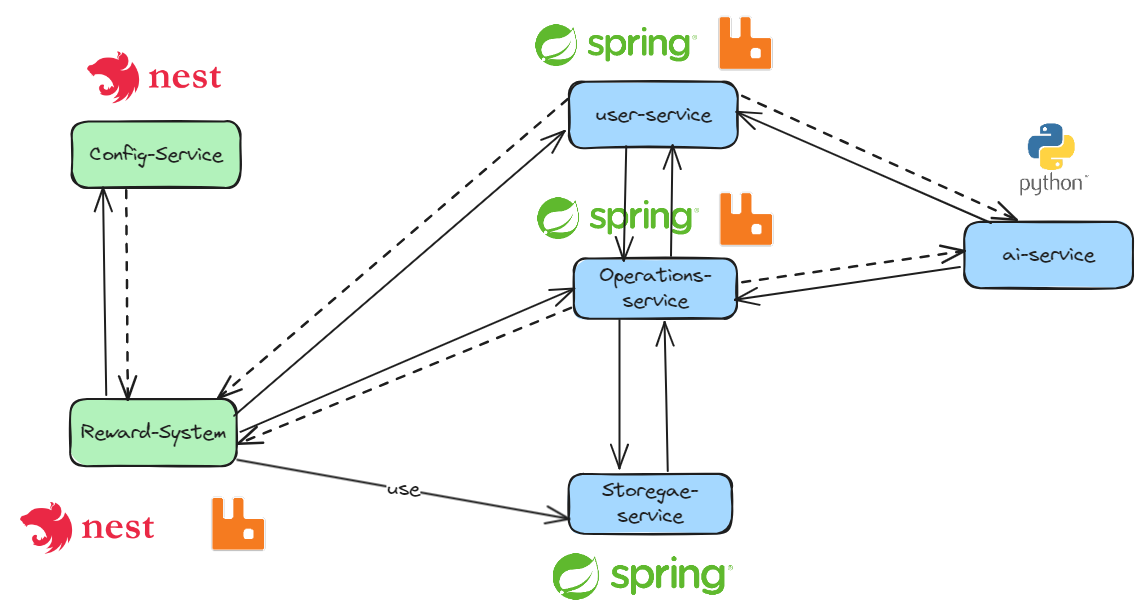
\includegraphics[width=1\textwidth]{src/assets/diagrams/microservicesComm.png}
    \caption{Communication Overview of Microservices}
    \label{fig:microservices}
\end{figure}

\begin{itemize}
    \item \textbf{Config-Service}\index{Config-Service}: The \textbf{Config-Service} stores and manages various configurations required by different microservices, including RabbitMQ configurations, achievement configurations, and translations.
    
    \item \textbf{Reward-System}\index{Reward-System}: The \textbf{Reward-System} handles user rewards and incentives, interacting with other microservices to track activities and assign rewards based on predefined rules.
\end{itemize}

\section{Software Architecture}

The architecture of our application is designed to promote scalability, maintainability, and efficiency. We utilize a combination of server-side and client-side frameworks to achieve these goals. The primary frameworks used are NestJS for the backend and ReactJS for the frontend.

\subsection{Server-side Technology}
This section delves into the technology considerations for the backend part of our solution and the employed internal architectural pattern.

\subsubsection*{NestJS Framework}
NestJS emerged as the backend technology for our project. NestJS is a progressive Node.js framework for building efficient, reliable, and scalable server-side applications. It is built with and fully supports TypeScript while still enabling developers to code in pure JavaScript. NestJS incorporates many modern programming paradigms and practices, such as modularization, dependency injection, and a strong emphasis on testability.

NestJS offers several core capabilities:
\begin{itemize}
    \item \textbf{Modular Architecture}: Helps in organizing the application into cohesive blocks of functionality, encapsulating related components such as controllers, services, and providers.
    \item \textbf{Dependency Injection}: Facilitates the development of loosely coupled modules.
    \item \textbf{Extensibility}: Supports a wide range of plugins and integrations, enhancing the framework's capabilities.
\end{itemize}

\subsubsection*{NestJS Flow Architecture}
NestJS uses a modular architecture where each module is a cohesive block of functionality. The primary components in this architecture are:

\begin{itemize}
    \item \textbf{Modules}: These are the basic building blocks of a NestJS application. Modules help in organizing the application into cohesive blocks of functionality. Each module encapsulates related components such as controllers, services, and providers.
    \item \textbf{Controllers}: Controllers handle incoming HTTP requests and return responses to the client. They are responsible for orchestrating the overall flow of the application.
    \item \textbf{Services}: Services contain the business logic and are responsible for performing operations like data processing and communication with the database.
    \item \textbf{Providers}: Providers are classes that can be injected as dependencies. They serve as a bridge to encapsulate various operations, services, and logic.
\end{itemize}

Below \ref{fig:mvc-diagram} is a diagram that illustrates the general architecture of NestJS following the MVC (Model-View-Controller) pattern:

\begin{figure}[H]
    \centering
    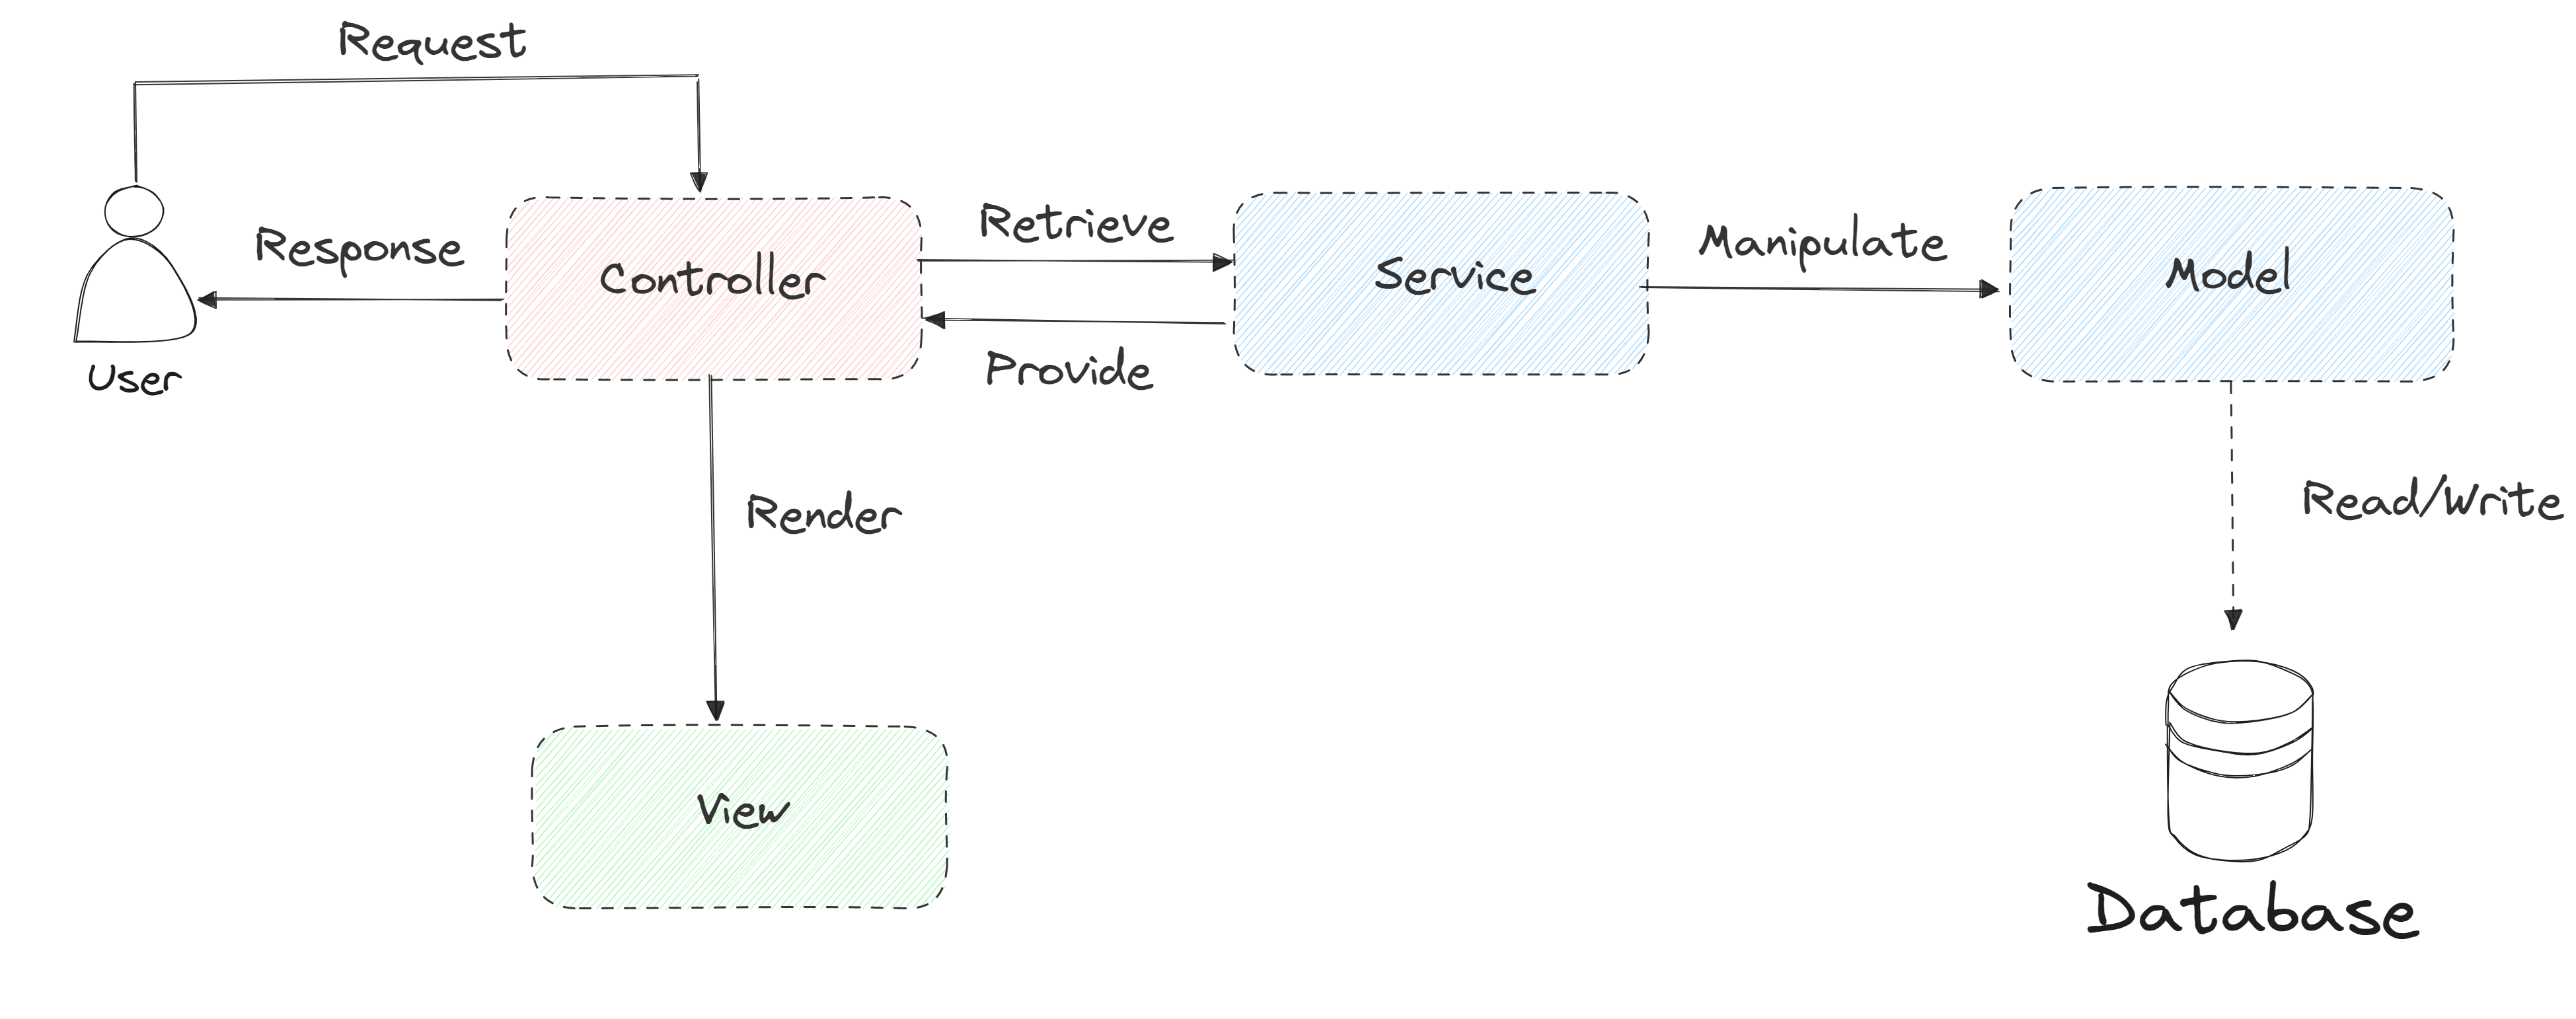
\includegraphics[width=\textwidth]{src/assets/diagrams/mvcDiagram.png}
    \caption{NestJS MVC Diagram}
    \label{fig:mvc-diagram}
\end{figure}

In this diagram:
\begin{itemize}
    \item The \textbf{Controller} handles the incoming request from the user, retrieves or manipulates data using the \textbf{Service}, and then sends back the appropriate response.
    \item The \textbf{Service} interacts with the \textbf{Model} to perform CRUD operations on the database.
    \item The \textbf{Model} represents the structure of the database and handles data reading and writing.
\end{itemize}

\subsection{Client-side Technology}
This section illustrates the chosen technology for the client side of our solution and the adopted internal architectural pattern.
\subsubsection*{ReactJS Framework}
For the user-facing part of our solution, we have selected the ReactJS frontend framework. ReactJS, developed and maintained by Facebook, is a JavaScript library for building user interfaces. It promotes a component-based architecture, which enhances reusability and manageability of the codebase \cite{ReactUpAndRunning}.

ReactJS offers several core capabilities:
\begin{itemize}
    \item \textbf{Component-Based Architecture}: Allows building encapsulated components that manage their own state, then compose them to make complex UIs.
    \item \textbf{Declarative Syntax}: Makes it easier to reason about the application and aims to be both efficient and flexible.
    \item \textbf{Virtual DOM}: Optimizes rendering by only updating components that have changed \cite{ProReact}.
\end{itemize}

\subsubsection*{ReactJS Architectural Pattern}
The architecture of a ReactJS application relies on certain fundamental concepts \cite{ReactUpAndRunning}:
\begin{itemize}
    \item \textbf{Components}: Define views, which are sets of screen elements that React can choose among and modify according to the program logic and data.
    \item \textbf{State and Props}: Components use state to manage their data internally and props to receive data from parent components.
    \item \textbf{Lifecycle Methods}: React provides lifecycle methods that can be used to perform actions at specific points in a component's life.
    \item \textbf{Event Handling}: React allows handling user inputs and interactions with event handlers.
\end{itemize}
\subsection{Database}

Selecting the appropriate database is a pivotal decision in our system design. After careful consideration, we’ve chosen to employ MongoDB. This choice is driven by the following criteria:

\begin{itemize}
    \item \textbf{Scalability}: MongoDB offers horizontal scalability, making it easier to manage large volumes of data and high-velocity workloads \cite{MongoDBTheDefinitiveGuide}.
    \item \textbf{Flexibility}: As a NoSQL database, MongoDB allows for a flexible schema design, which is particularly useful for evolving data models and handling unstructured data \cite{LearningNoSQL}.
    \item \textbf{Performance}: MongoDB provides high performance for read and write operations, which is critical for applications requiring fast data access and real-time analytics \cite{MongoDBAppliedDesignPatterns}.
    \item \textbf{Ease of Use}: MongoDB's document-oriented storage format aligns well with the JSON format, simplifying data exchange between the backend (NestJS) and frontend (ReactJS) \cite{MongoDBTheDefinitiveGuide}.
    \item \textbf{Community and Ecosystem}: MongoDB has a robust community and a rich ecosystem of tools and libraries, which support and streamline the development process \cite{LearningNoSQL}.
\end{itemize}

By leveraging MongoDB, we ensure that our application can efficiently handle current and future data requirements, providing a robust foundation for scalability and performance \cite{MongoDBAppliedDesignPatterns}.

\section{Design}
This phase of the project builds upon our foundational work to refine and expand the architecture of our reward system. We delve into key considerations, decisions, and enhancements introduced in this release, focusing particularly on how our models support the reward functionalities.


\subsection{Static modeling}
The static modeling phase has been pivotal in defining the core structure of our reward system. We have continued to refine our data models and database schema to align with our evolving functional requirements and business rules.


\subsubsection*{Domain model}
We have structured our reward system around four primary classes: RewardLog, UserRewards, and Achievement. These classes are designed to seamlessly interact within our system to facilitate efficient reward management and user engagement through achievements.
\\

\begin{longtable}{ | m{0.3\textwidth} | m{0.645\textwidth} | }
    \caption{Classes description}                                                                                                               \\
    \hline
    \textbf{Class name}    & \textbf{Description}                                                                                               \\
    \hline
    \endfirsthead
    \hline
    \textbf{Class name}    & \textbf{Description}                                                                                               \\
    \hline
    \endhead
    \endfoot
    \hline
    \endlastfoot
    RewardLog                 & This class models individual reward transactions, capturing details like  reward type (XP, token), amount, and the source of the reward (e.g., completing a task or manual adjustment). \\
    \hline
    UserRewards               & This class models the cumulative rewards and achievements for a user, providing a comprehensive overview of their progress and tokens. \\
    \hline
    Achievement              & This class models the achievements that users can earn, including the criteria for earning them and the rewards associated with them. \\
    \hline
    Rank                     & This class models the various ranks users can achieve. Each rank includes a label , the levels required to reach the rank, and a description that highlights the significance of the rank. This class helps track user progression and assigns appropriate ranks based on their XP levels. \\
    \hline
\end{longtable}
The following figure illustrates the class diagram of our reward system, which is a crucial part of our application. This diagram visually represents the structure of the reward system, detailing the various classes, their attributes, and the relationships between them:

\begin{itemize}
    \item \texttt{User}: Linked to \texttt{UserRewards} and \texttt{Packet}, representing multiple rewards and packets.
    \item \texttt{Achievement}: Contains information about achievements, such as ID, name, reward, and description.
    \item \texttt{RewardLog}: Records reward transactions, linking users to achievements and packets.
    \item \texttt{UserAchievementSubdocument}: Subdocument within a user, detailing progress on each achievement.
    \item \texttt{SubCompany}: Shows the connection with \texttt{User}, indicating hierarchical structure.
    \item \texttt{Rank}: Defines ranks within the system with unique IDs and descriptions.
    \item \texttt{UserRewards}: Aggregates a user's rewards, including XP, tokens, and ban status.
\end{itemize}

This class diagram provides a comprehensive overview of the reward system's architecture, enabling a clear understanding of the interactions between different components (see Figure \ref{fig:reward_system-class}).

\begin{figure}[H]
    \centering
    \makebox[\textwidth]{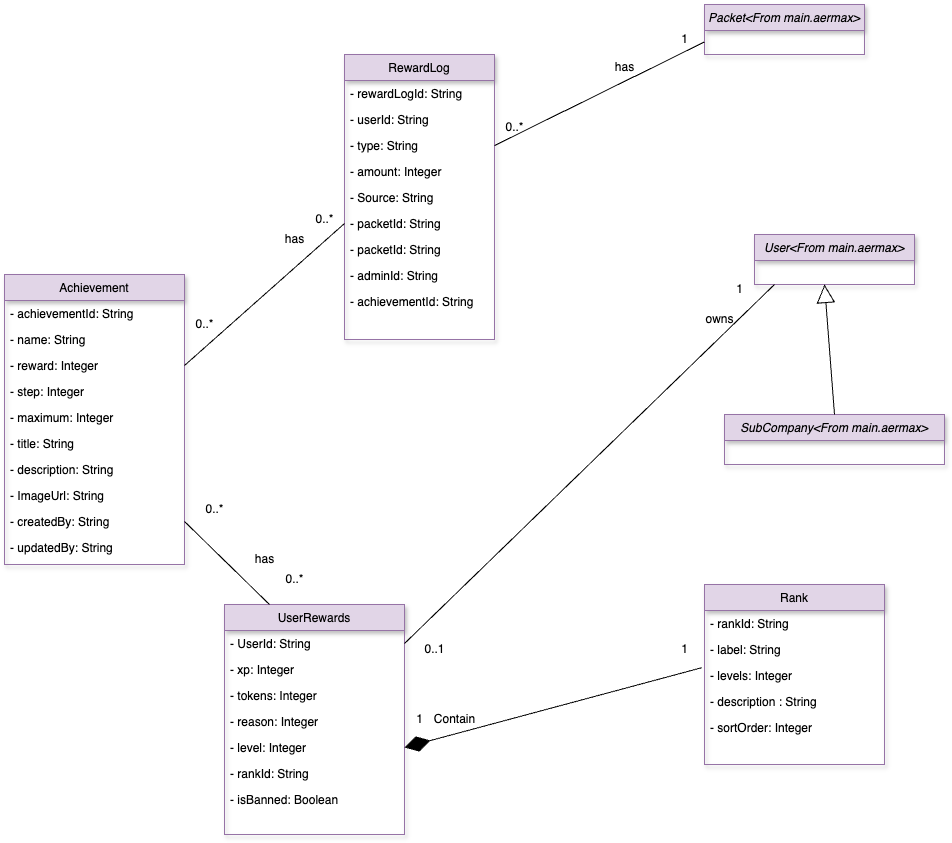
\includegraphics[width=16cm, height=19cm, keepaspectratio]{src/assets/diagrams/reward--system-classDiagram.drawio.png}}
    \caption{Reward system class diagram}
    \label{fig:reward_system-class}
\end{figure}

\subsubsection*{Data dictionary}
In the table \ref{database-architecture}, we provide a comprehensive overview of the essential data elements
that will define our entities and relationships for the second release.


\begin{landscape}
    \begin{longtable}{ | m{0.225\textwidth} | m{0.28\textwidth} | m{0.55\textwidth} | m{0.15\textwidth} | m{0.2\textwidth} | }
        \caption{Data Dictionary of User Rewards Management System}   \label{database-architecture}                                                                                                                                                                  \\
        \hline
        \textbf{Entity}                                                  & \textbf{Field}                            & \textbf{Description}                                                 & \textbf{Type} & \textbf{Constraints}          \\
        \hline
        \endfirsthead
        \hline
        \textbf{Entity}                                                  & \textbf{Field}                            & \textbf{Description}                                                 & \textbf{Type} & \textbf{Constraints}          \\
        \hline
        \endhead
        \hline
        \endfoot
        \endlastfoot
        \multirow[t]{8}{5em}{\textbf{RewardLog}}                         & \texttt{id}                               & Reward log's unique identifier                                       & objectId      & Primary key \newline Not null \\
        \cline{2-5}
                                                                         & \texttt{userId}                           & User ID associated with the reward                                   & string        & Not null                      \\
        \cline{2-5}
                                                                         & \texttt{type}                             & Type of reward (XP, TOKEN)                                           & string        & Not null                      \\
        \cline{2-5}
                                                                         & \texttt{amount}                           & Amount of reward                                                     & double        & Not null                      \\
        \cline{2-5}
                                                                         & \texttt{source}                           & Source of the reward (CLOSE\_PACKET, MANUAL\_ADJUSTMENT, ACHIEVEMENT) & string       & Not null                      \\
        \cline{2-5}
                                                                         & \texttt{packetId}                         & Packet ID, if applicable                                             & string        &                               \\
        \cline{2-5}
                                                                         & \texttt{adminId}                          & Admin ID who issued the reward, if applicable                        & string        &                               \\
        \cline{2-5}
                                                                         & \texttt{achievementId}                    & Achievement ID related to the reward, if applicable                  & objectId      &                               \\
        \hline
        \multirow[t]{10}{5em}{\textbf{UserRewards}}                      & \texttt{id}                               & User rewards' unique identifier                                      & objectId      & Primary key \newline Not null \\
        \cline{2-5}
                                                                         & \texttt{userId}                           & User ID                                                              & string        & Not null                      \\
        \cline{2-5}
                                                                         & \texttt{xp}                               & Experience points of the user                                        & double        & Default: 0                    \\
        \cline{2-5}
                                                                         & \texttt{tokens}                           & Tokens owned by the user                                             & double        & Default: 0                    \\
        \cline{2-5}
                                                                         & \texttt{reason}                           & Reason for the last update                                           & string        & Default: ''                   \\
        \cline{2-5}
                                                                         & \texttt{level}                            & Level of the user                                                    & double        & Default: 0                    \\
        \cline{2-5}
                                                                         & \texttt{rank}                             & Rank of the user                                                     & objectId      &                               \\
        \cline{2-5}
                                                                         & \texttt{achievements}                     & List of achievements the user has earned                             & array         & Default: []                   \\
        \cline{2-5}
                                                                         & \texttt{isBanned}                         & Whether the user is banned                                           & bool          & Default: false                \\
        \cline{2-5}
                                                                         & \texttt{createdAt}                        & Creation date                                                        & date          &                               \\
        \cline{2-5}
                                                                         & \texttt{updatedAt}                        & Last update date                                                     & date          &                               \\
        \hline
        \multirow[t]{10}{5em}{\textbf{Achievement}}                      & \texttt{id}                               & Achievement's unique identifier                                      & objectId      & Primary key \newline Not null \\
        \cline{2-5}
                                                                         & \texttt{name}                             & Name of the achievement                                              & string        & Not null                      \\
        \cline{2-5}
                                                                         & \texttt{reward}                           & Reward amount                                                        & double        & Default: 0                    \\
        \cline{2-5}
                                                                         & \texttt{step}                             & Current step of the achievement                                      & double        & Default: 1                    \\
        \cline{2-5}
                                                                         & \texttt{maximum}                          & Maximum value of the achievement                                     & double        & Default: 1                    \\
        \cline{2-5}
                                                                         & \texttt{title}                            & Title of the achievement                                             & string        & Not null                      \\
        \cline{2-5}
                                                                         & \texttt{description}                      & Detailed description of the achievement                              & string        & Not null                      \\
        \cline{2-5}
                                                                         & \texttt{imageUrl}                         & URL of the image associated with the achievement                     & string        & Nullable                      \\
        \cline{2-5}
                                                                         & \texttt{createdBy}                        & ID of the user who created the achievement                           & string        & Not null                      \\
        \cline{2-5}
                                                                         & \texttt{updatedBy}                        & ID of the user who last updated the achievement                      & string        & Not null                      \\
        \hline
        \multirow[t]{4}{5em}{\textbf{Rank}}                              & \texttt{id}                               & Rank's unique identifier                                             & objectId      & Primary key \newline Not null \\
        \cline{2-5}
                                                                         & \texttt{label}                            & Label of the rank                                                    & string        & Not null                      \\
        \cline{2-5}
                                                                         & \texttt{levels}                           & Levels required to reach the rank                                    & double        & Not null                      \\
        \cline{2-5}
                                                                         & \texttt{description}                      & Description of the rank                                              & string        & Not null                      \\
        \hline
    \end{longtable}
\end{landscape}

\subsubsection*{data model}
In this section, I will present the document model for our MongoDB database. These diagrams will visually represent our data structures and their relationships. Due to extensive interactions with other microservices, there are fewer direct relationships within the MongoDB entities. This design minimizes internal dependencies, relying on microservice communication to handle complex interactions, thereby enhancing system flexibility and scalability.
\noindent The figure \ref{fig:database-architecture} illustrates the entity-relationship diagram.

\begin{figure}[H]
    \centering
    \makebox[\textwidth]{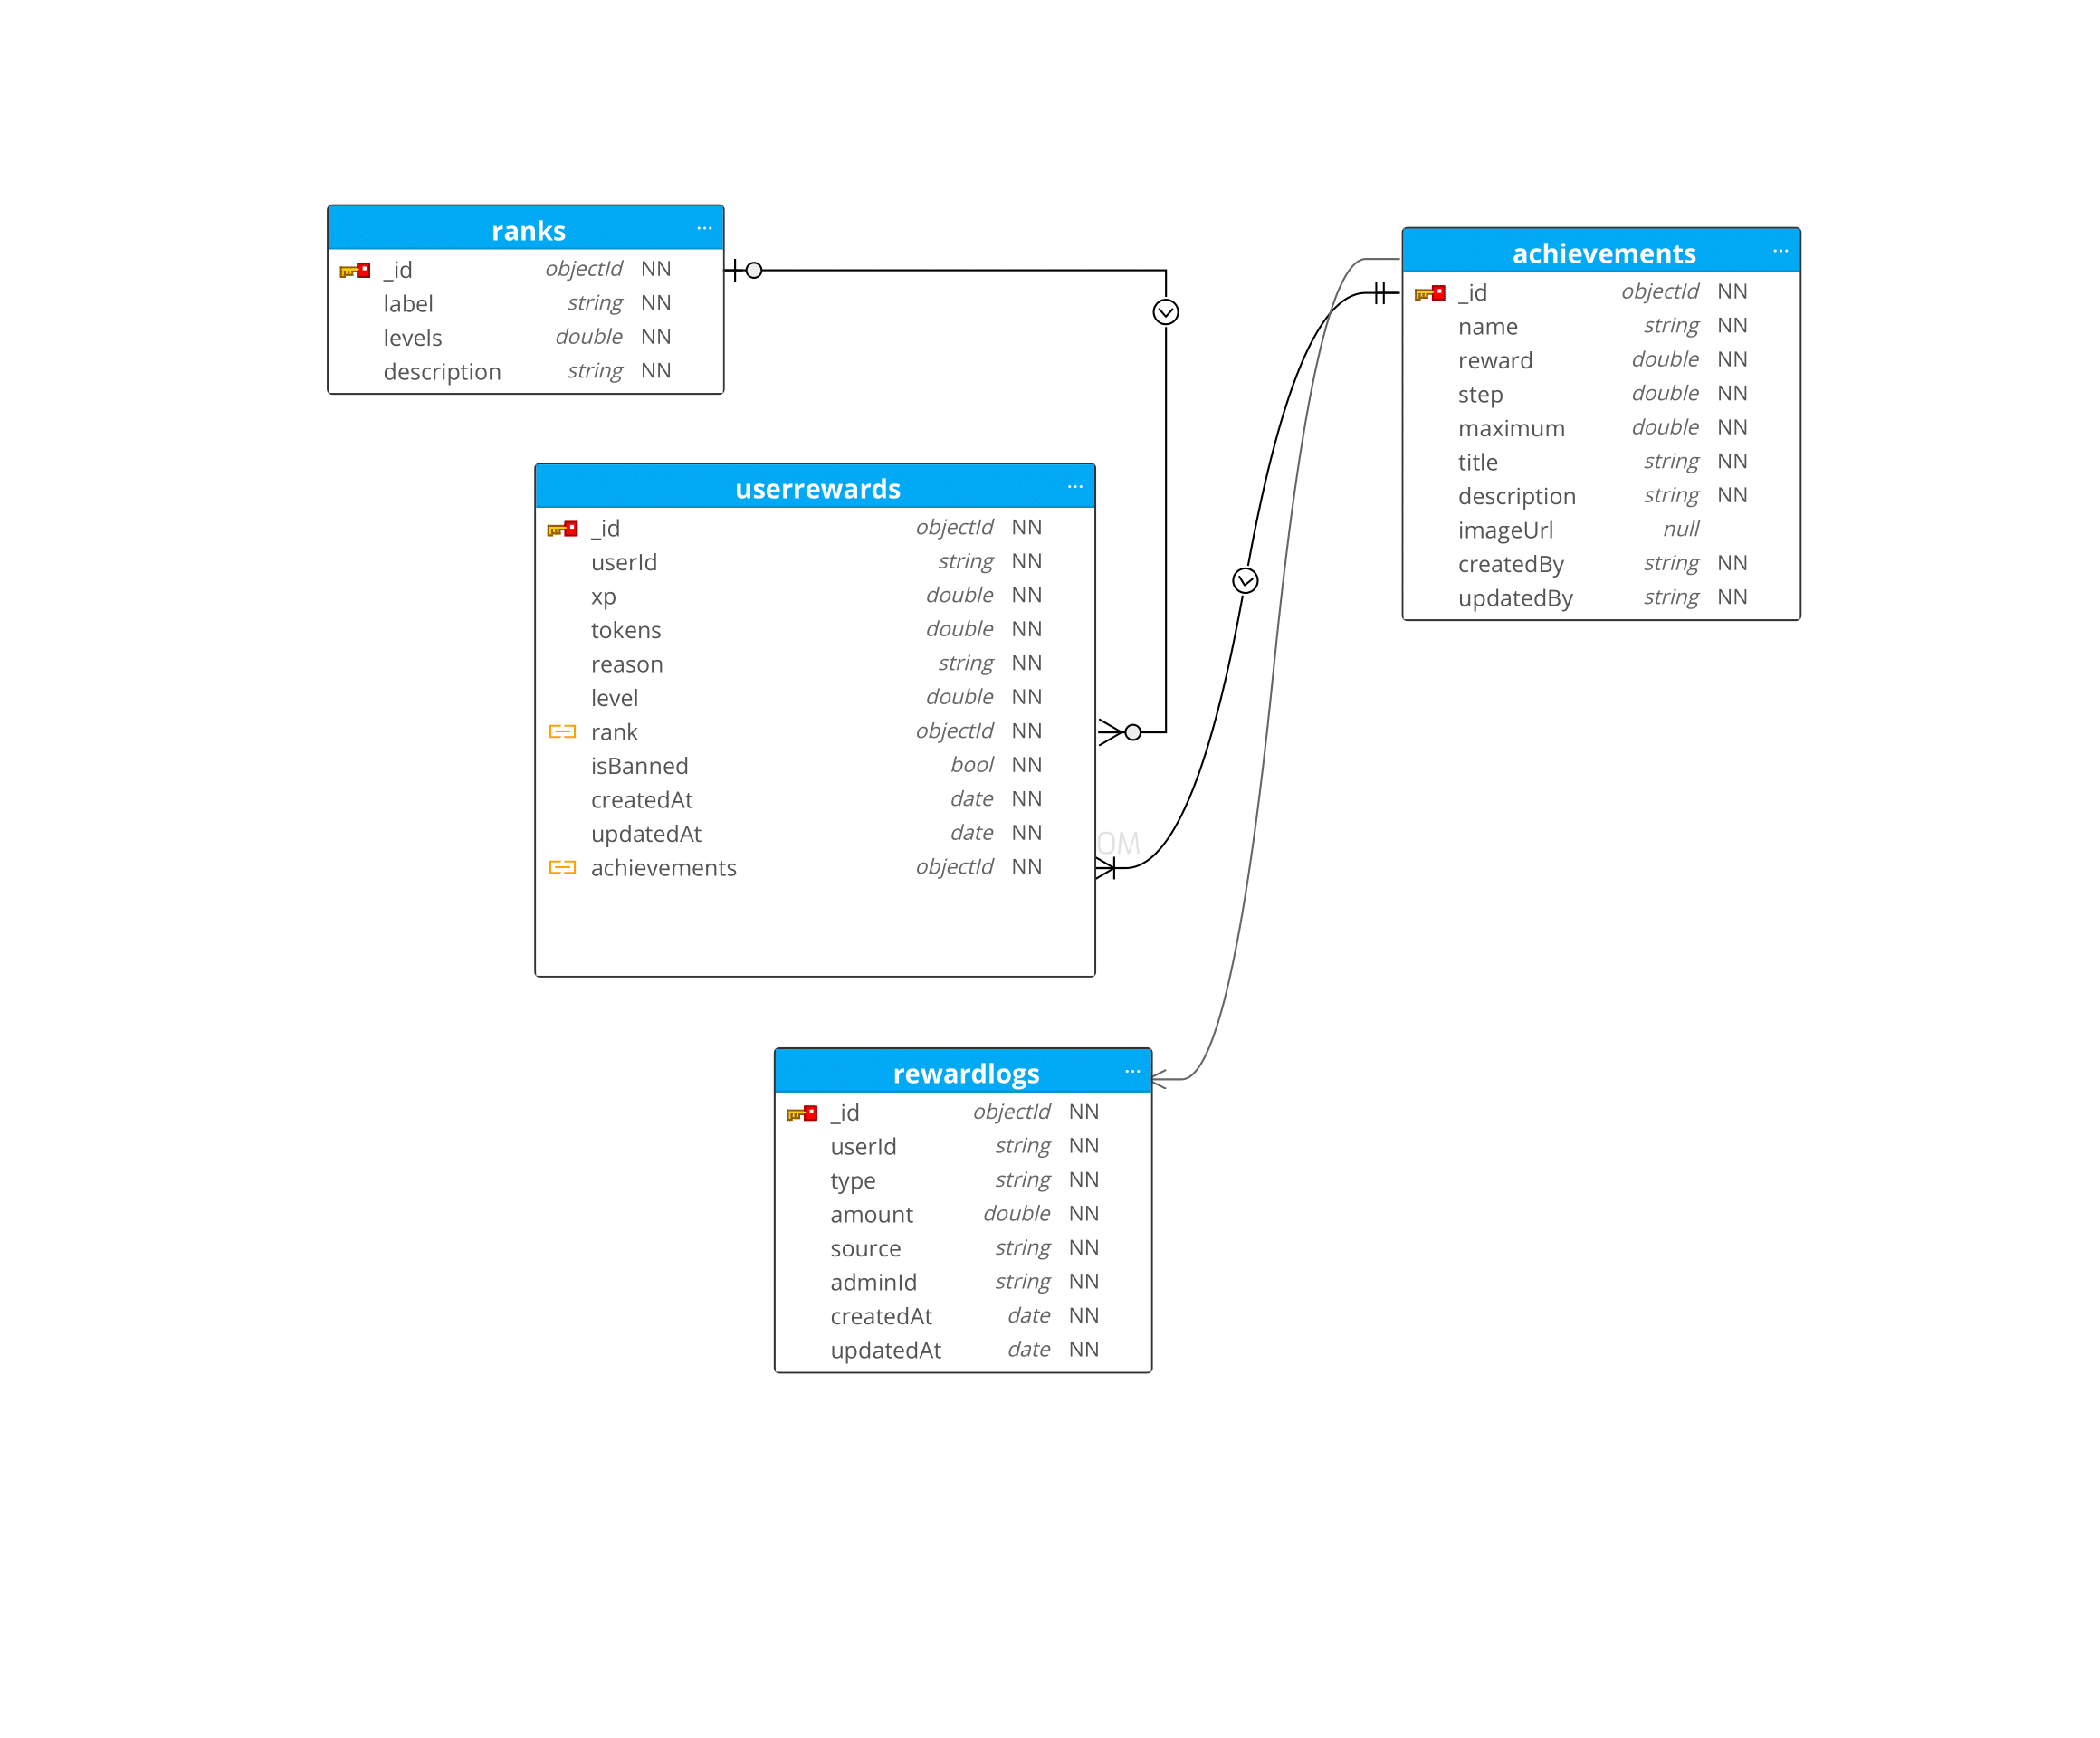
\includegraphics[width=16cm, height=12cm, keepaspectratio]{src/assets/diagrams/RewardSystemC-1.png}}
    \caption{Document oriented data model}
    \label{fig:database-architecture}
\end{figure}

\subsection{Dynamic modeling}
In this section, we utilize UML sequence diagrams to illustrate the dynamic aspects of our software solution. These diagrams visually map out the interactions and communication patterns between various components and actors within our system. By examining these sequences, we aim to clarify the flow of information, the sequence of operations, and the coordination among different elements in our software architecture.
\subsubsection{Sequence diagram for Admin XP Increment Process}

This sequence diagram illustrates the process by which an admin increments a user's XP in the system. The diagram showcases the interactions and communication patterns between the front-end components, various backend services, and the database. It details the steps involved, from the admin's action to the final update in the user rewards and the corresponding log entries, highlighting error handling for scenarios like user not found, invalid user ID or amount, and access forbidden. The diagram emphasizes the flow of information, the order of operations, and the coordination between different system elements to achieve the desired outcome.

\noindent The figure \ref{fig:admin-xp-increment-process} illustrates the sequence diagram for the admin XP increment process.

\subsubsection{Sequence diagram for closing a packet}

To close a packet, a subcontractor selects and confirms the action from the front-end interface. The front end sends a request to the backend to update the packet status.

The backend controller processes and validates the request, then interacts with the service layer to update the packet status and save changes to the database. Upon successful update, a completion notification is published, triggering updates to the subcontractor's achievements and reward points, which are logged accordingly.

The controller then sends a response back to the front end, confirming the packet has been closed. The front end updates the interface to display the new packet status and reward information.

\noindent The figure \ref{fig:seq-close-packet} illustrates the sequence diagram for closing a packet.

\begin{landscape}
    \begin{figure}[H]
        \centering
        \makebox[\textwidth]{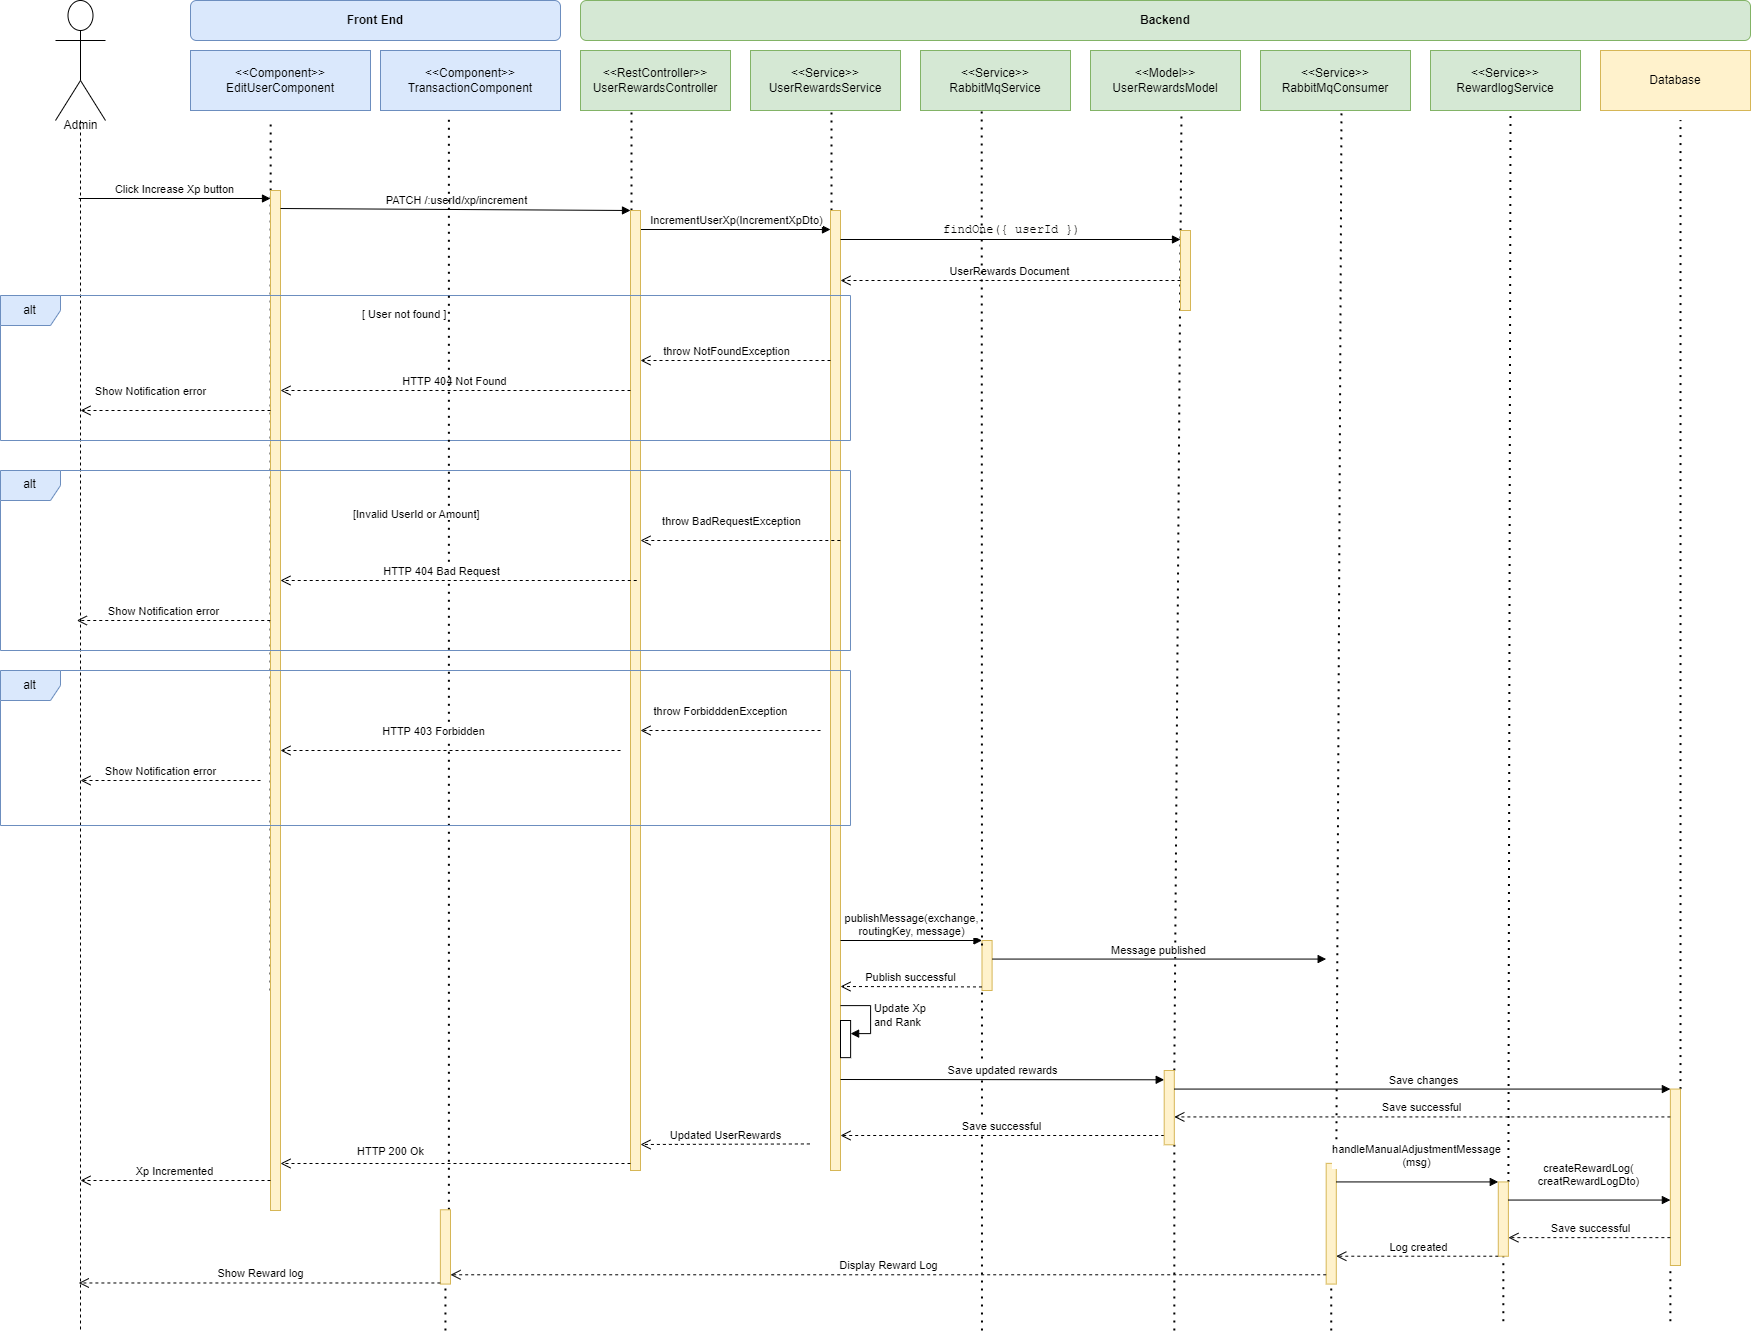
\includegraphics[width=24cm , height=15cm]{src/assets/diagrams/AdminIncreaseXp.png}}
        \caption{Admin XP Increment Process}
        \label{fig:admin-xp-increment-process}
    \end{figure}
\end{landscape}

\begin{landscape}
    \begin{figure}[H]
        \centering
        \makebox[\textwidth]{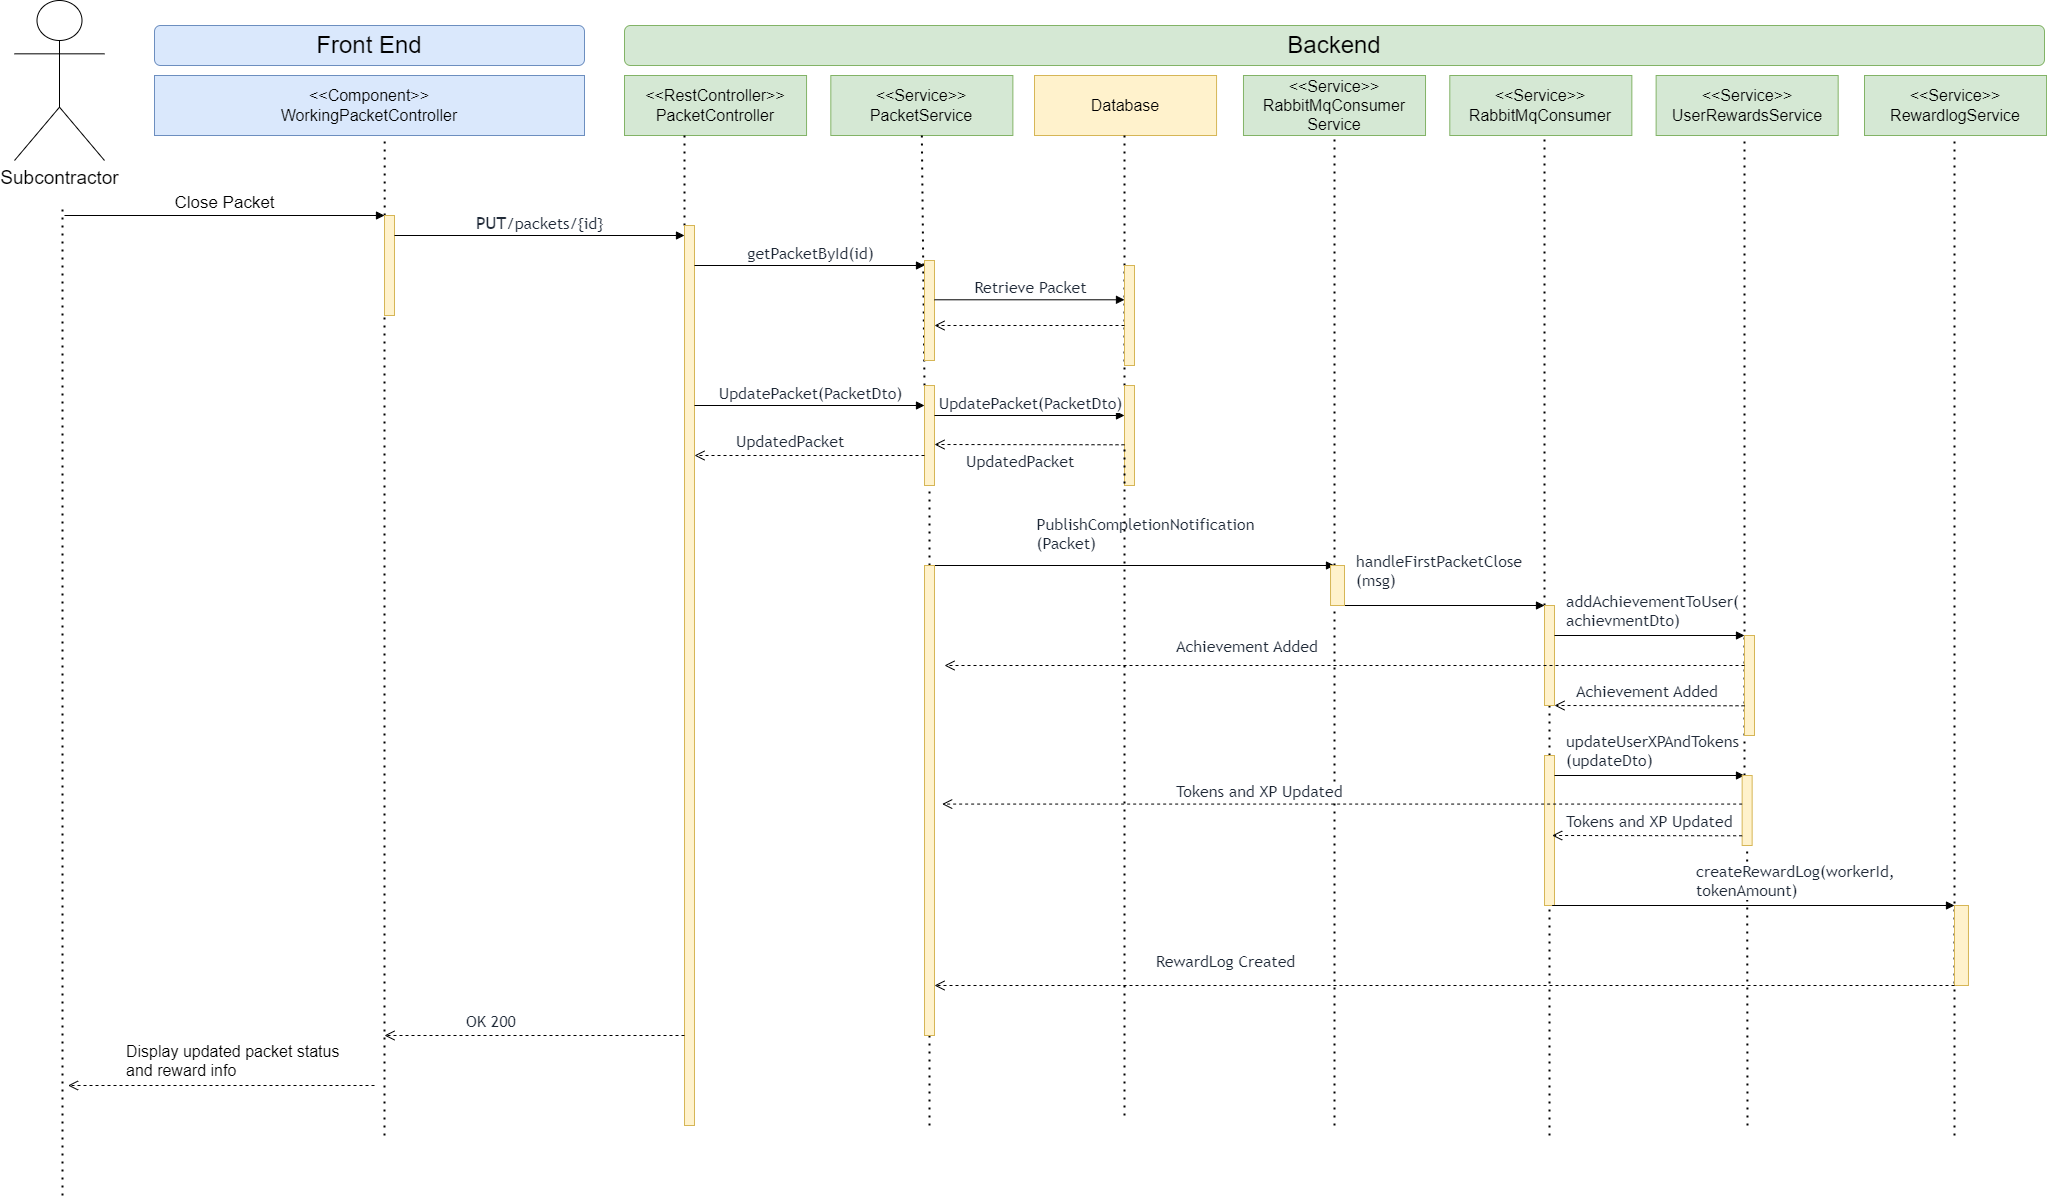
\includegraphics[width=24cm , height=15cm]{src/assets/diagrams/ClosePacketDiagram.png}}
        \caption{Sequence diagram for closing a packet}
        \label{fig:seq-close-packet}
    \end{figure}
\end{landscape}


\section{Detailed Design}
To provide a comprehensive understanding of feature implementations, we will illustrate the classes that are directly tied to the reward system. This focused diagram serves as an extension of our system architecture, detailing the interactions and relationships between the various components involved in managing user rewards, achievements, and related data. 

The diagram encompasses several key areas:

\begin{itemize}
    \item \textbf{Domain Entities}: Represent specific concepts within the reward system, such as logs, ranks, user rewards, and achievements.
    
    \item \textbf{Data Transfer Objects (DTOs)}: Facilitate data transfer between different application layers, encapsulating data required for specific operations.
    
    \item \textbf{Repositories}: Define methods for interacting with the database to retrieve and store data related to rewards, ranks, logs, and user rewards.
    
    \item \textbf{Services}: Implement business logic, using repositories to perform operations like creating achievements and updating user rewards.
    
    \item \textbf{Controllers}: Define API endpoints for interacting with the reward system, handling incoming requests, and returning responses.
    
    \item \textbf{Mappers}: Convert data between entities and DTOs, ensuring correct data formatting between the database and application layers.
    
    \item \textbf{Validators}: Ensure input data meets required criteria before processing, maintaining data integrity and preventing errors.
    
    \item \textbf{Exceptions}: Handle specific error cases and provide meaningful error messages.
\end{itemize}

This detailed design provides a clear overview of how the reward system components interact and work together to manage user rewards effectively. By illustrating these classes and their relationships, we aim to give a thorough understanding of the reward system's implementation. The implementation is done using the NestJS framework, which allows for efficient and scalable development of server-side applications.

As shown in Figure \ref{fig:class-reward-system}, the diagram provides a detailed view of the classes involved in the reward system and their interactions.

\begin{landscape}
    \begin{figure}[H]
        \centering
        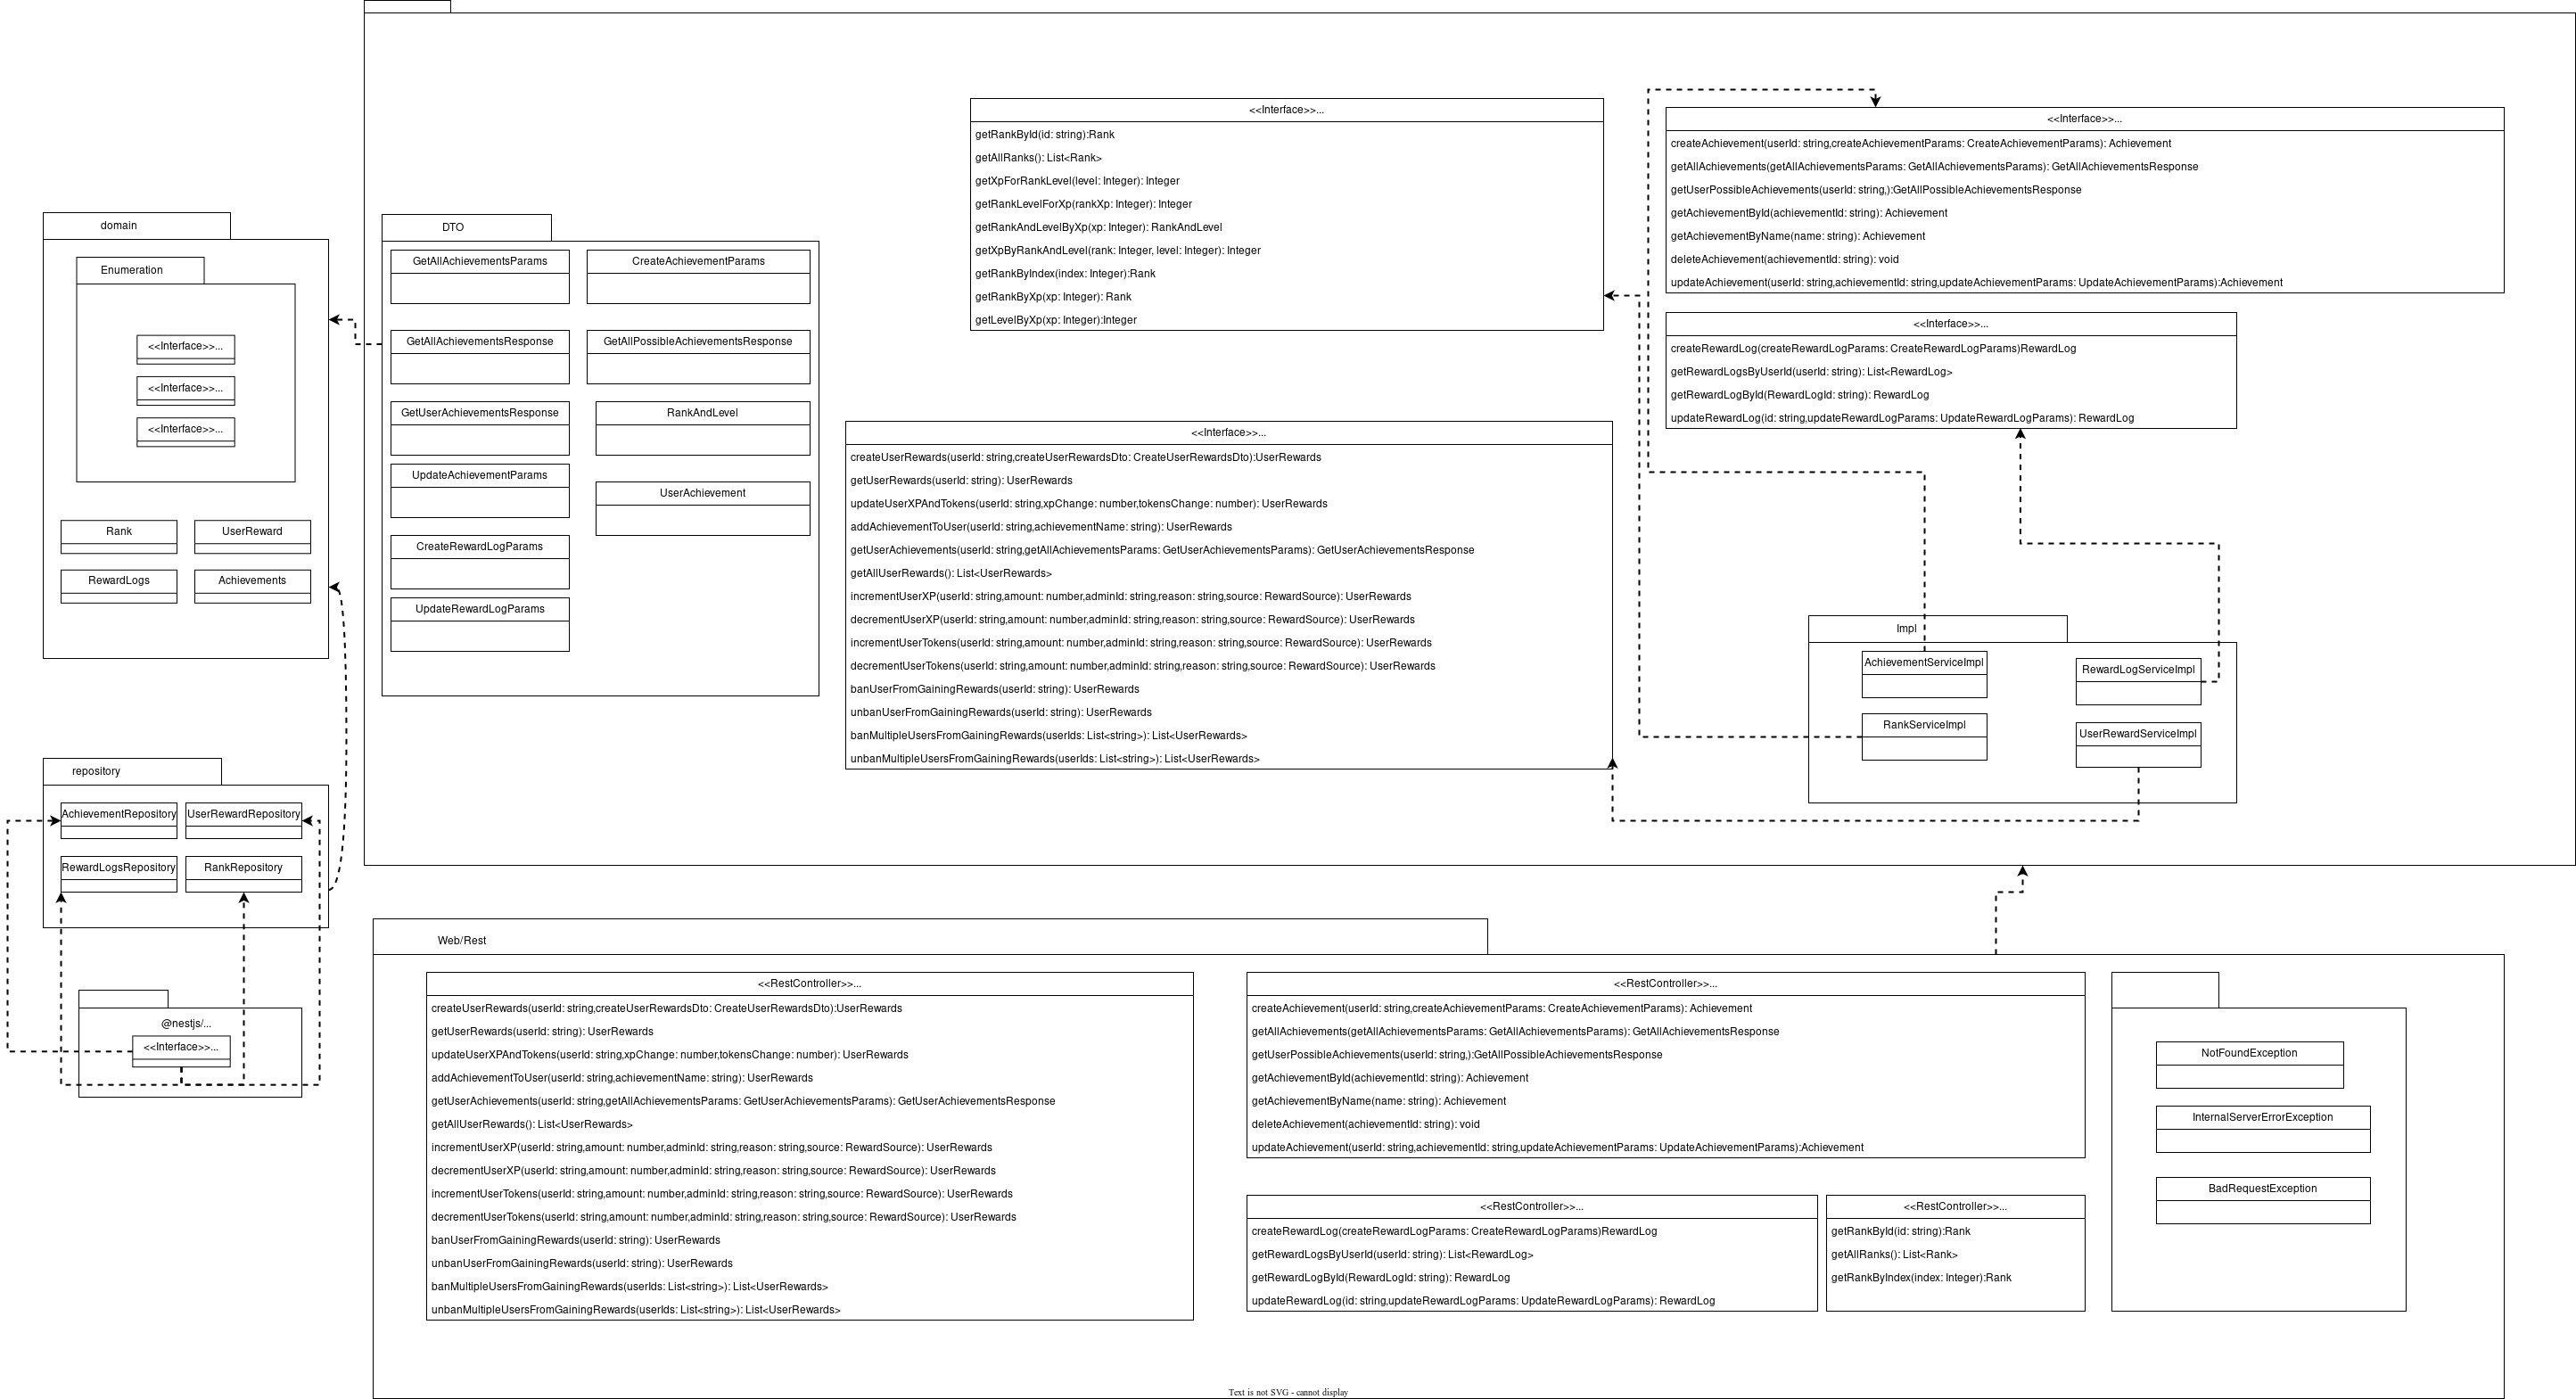
\includegraphics[width=24cm, height=15cm]{src/assets/diagrams/nestclass.png}
        \caption{Class diagram for the reward system components}
        \label{fig:class-reward-system}
    \end{figure}
\end{landscape}

\section{Message Broker: RabbitMQ}

In our project, we require a robust mechanism for managing communication between different microservices. This is where a message broker comes into play. A message broker helps in decoupling applications and enables them to communicate asynchronously. By using a message broker, we can ensure reliable delivery of messages, handle large volumes of messages, and improve the scalability and fault-tolerance of our system.

We chose RabbitMQ as our message broker due to its lightweight nature, ease of use, and strong support for various messaging patterns. RabbitMQ is an open-source message broker that implements the Advanced Message Queuing Protocol (AMQP). It supports multiple messaging protocols, has excellent documentation, and a large community.

\begin{itemize}
    \item \textbf{Decoupling}: It allows different parts of our system to communicate without being tightly coupled, which improves modularity and flexibility.
    \item \textbf{Scalability}: Helps in handling increased load by distributing messages across multiple consumers.
    \item \textbf{Reliability}: Ensures that messages are delivered even in the case of service failures.
    \item \textbf{Asynchronous Communication}: Enables services to process messages at their own pace without waiting for each other.
\end{itemize}

\begin{table}[H]
    \centering
    \begin{tabularx}{\linewidth}{|l|X|X|X|}
        \hline
        \textbf{Feature} & \textbf{RabbitMQ} & \textbf{Apache Kafka} & \textbf{ActiveMQ} \\ \hline
        Protocol Support & AMQP, MQTT, STOMP & Kafka Protocol & OpenWire, AMQP, STOMP, MQTT \\ \hline
        Message Persistence & Yes & Yes & Yes \\ \hline
        Throughput & Moderate & High & Moderate \\ \hline
        Latency & Low & Low & Low \\ \hline
        Use Case Suitability & General-purpose & High-throughput, event streaming & General-purpose \\ \hline
        Community Support & Large & Large & Medium \\ \hline
        Ease of Setup & Easy & Moderate & Moderate \\ \hline
        Documentation & Excellent & Excellent & Good \\ \hline
    \end{tabularx}
    \caption{Comparison of RabbitMQ with Other Message Brokers}
    \label{tab:message-broker-comparison}
\end{table}
We selected RabbitMQ because it provides a balanced mix of ease of use, reliability, and community support. It is suitable for general-purpose messaging and supports multiple protocols, which gives us flexibility. RabbitMQ's ease of setup and extensive documentation make it an excellent choice for our project, ensuring that we can implement and maintain it with minimal overhead.

As shown in Figure \ref{fig:rabbitmq-diagram}, the diagram provides an overview of how RabbitMQ is used in our system. The subcontractor closes a packet, which the `operations-service` produces as a message. This message is then published to an exchange in RabbitMQ, which routes it to the appropriate queue. The `reward-service` consumes the message from the queue to process the increment of tokens and XP.

\begin{figure}[H]
    \centering
    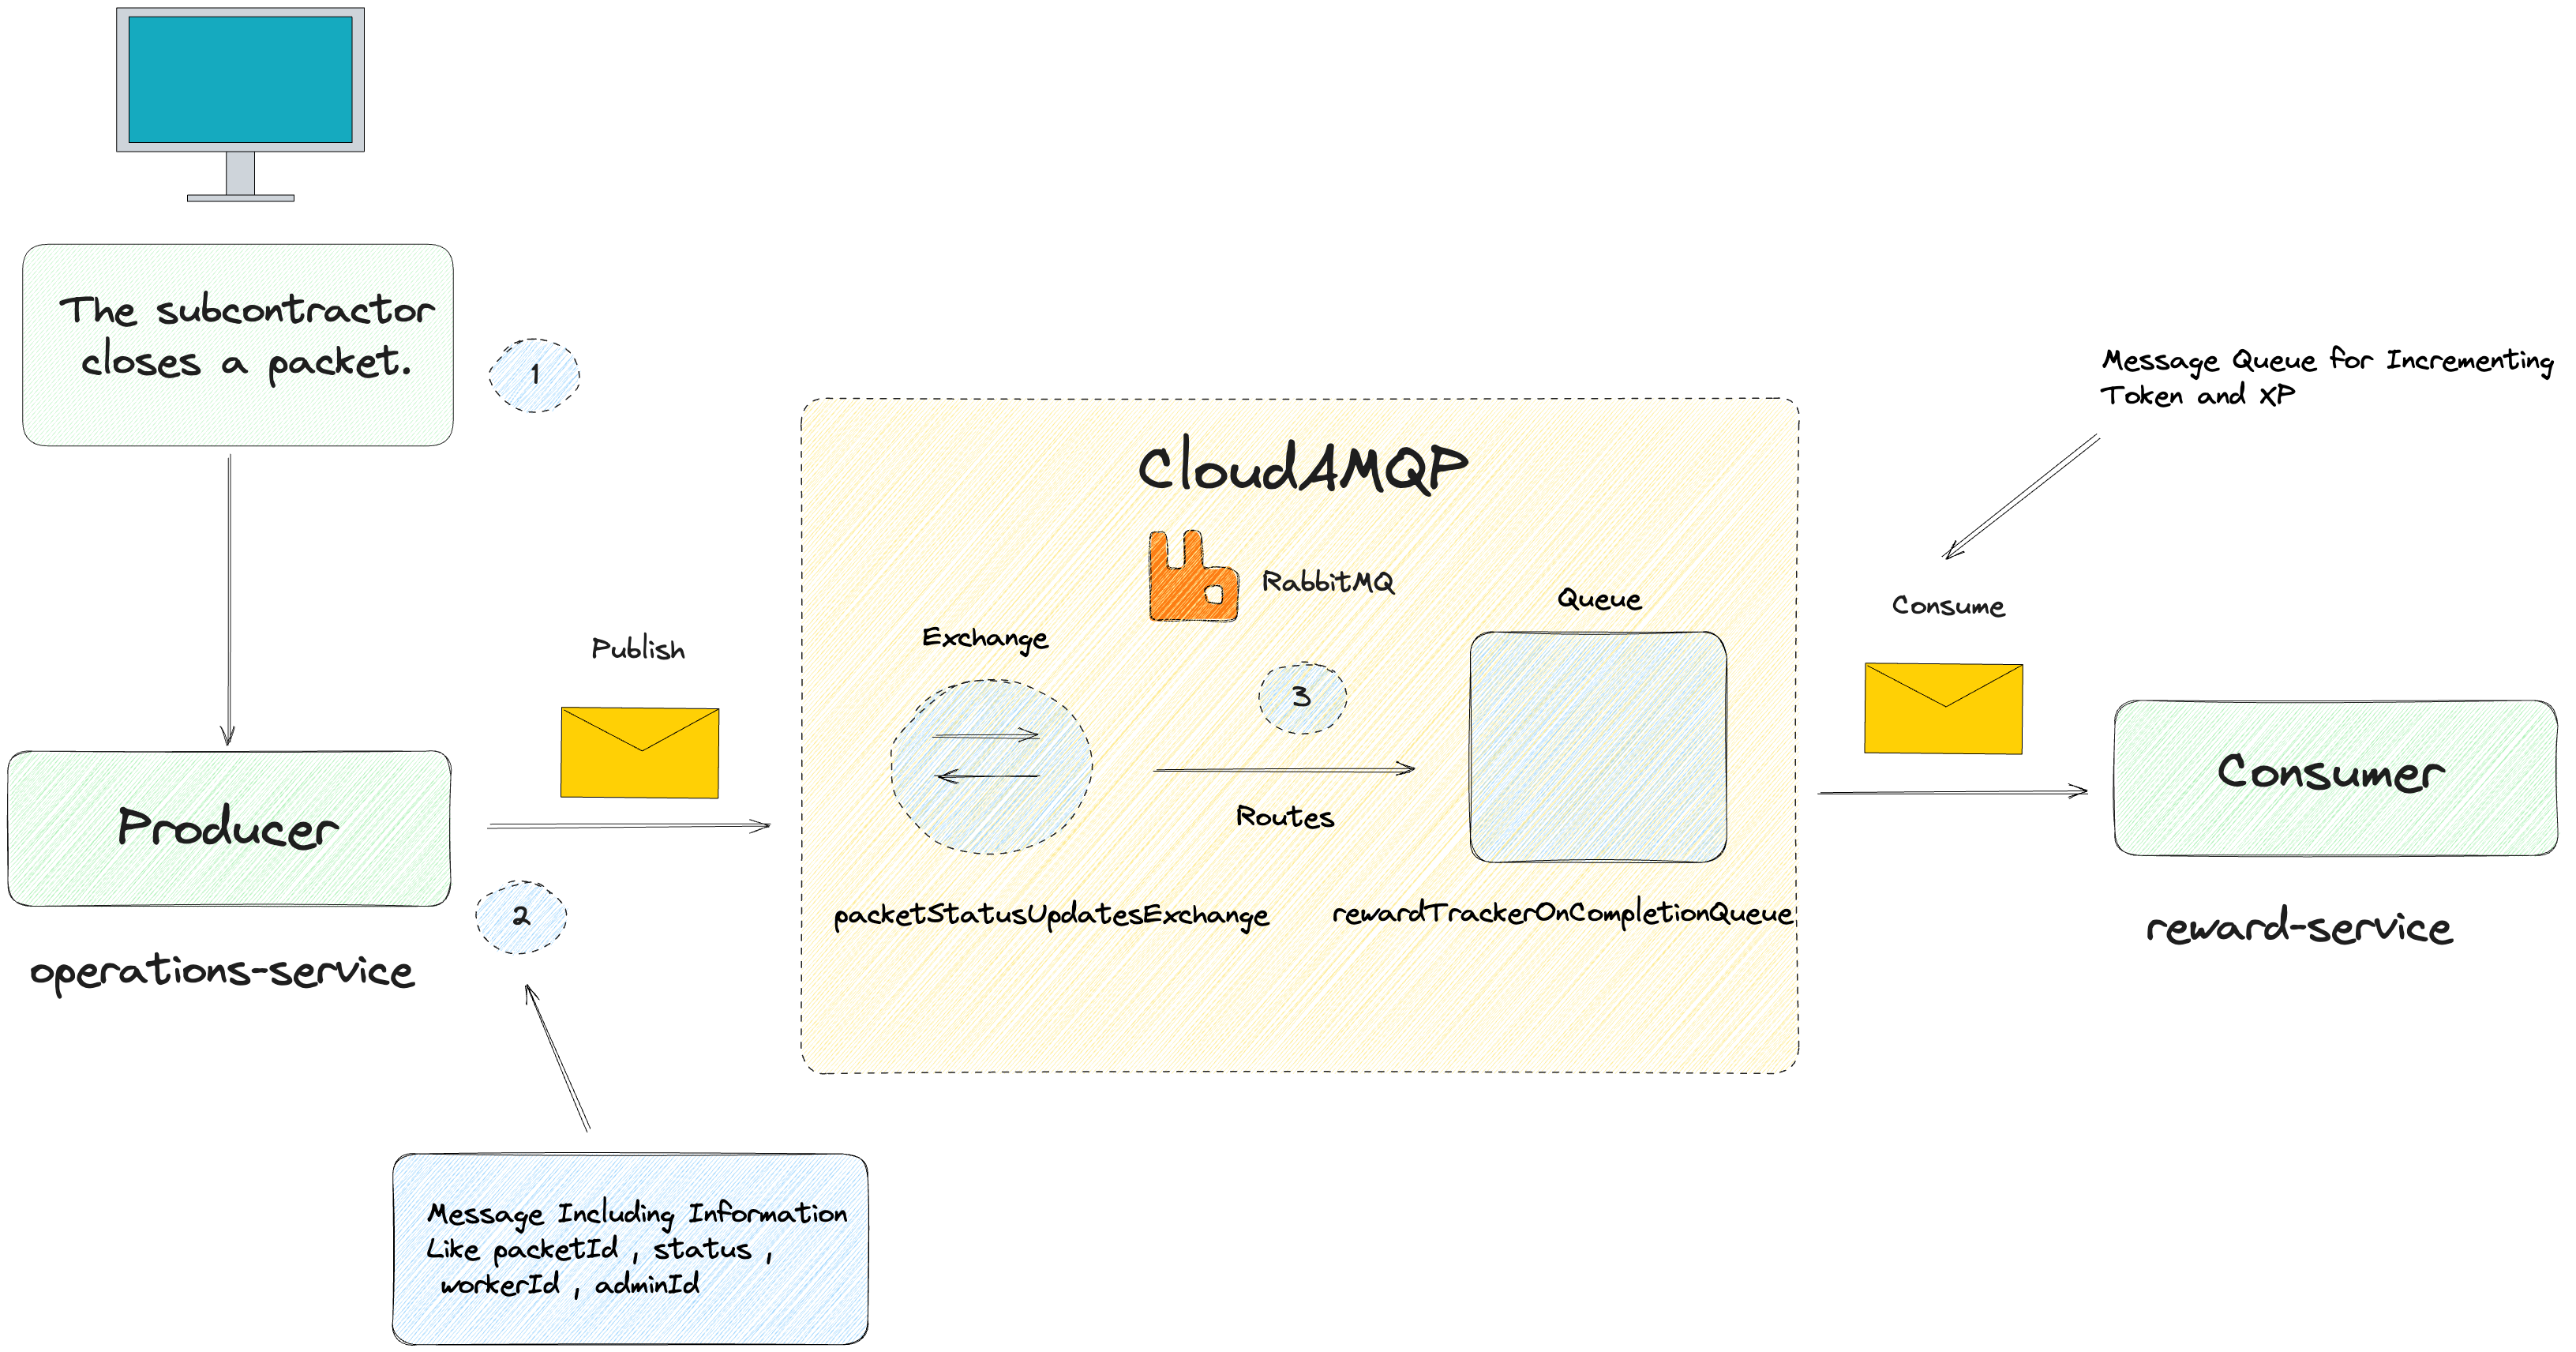
\includegraphics[width=\linewidth]{src/assets/diagrams/RabbitMqExplanation.png}
    \caption{Message flow using RabbitMQ in our system}
    \label{fig:rabbitmq-diagram}
\end{figure}

\setcounter{secnumdepth}{0}
\section{Conclusion}
In this chapter, we have explored the planning, design considerations, and implementation details of our reward system. We discussed the sprint backlog, specifications for various user stories, and the communication overview of our microservices. Detailed designs, including static and dynamic modeling, were provided to illustrate the interactions and relationships between the different components of the reward system. 

Furthermore, we introduced RabbitMQ as our chosen message broker, explaining its benefits, comparison with other message brokers, and its role in our system architecture.

In the next chapter, we will delve into the deployment and implementation aspects of the reward system, covering the steps and processes involved in bringing our designed solution into a live production environment.


 